\documentclass[11pt,a4paper]{article}
\usepackage[T1]{fontenc}
\usepackage{lmodern}
\usepackage[margin=2.2cm]{geometry}
\usepackage{graphicx}
\usepackage{float}
\usepackage{caption}
\usepackage{subcaption}
\usepackage{longtable}
\captionsetup{font=small,labelfont=bf}
\setlength{\parskip}{0.5em}
\setlength{\parindent}{0pt}
\usepackage[hidelinks,bookmarksnumbered]{hyperref}

\title{Value investing: buy-and-hold results}
\author{S\&P SmallCap 600, data as of 2026-10-31}
\date{}
\begin{document}
\maketitle
\begin{abstract}
Each January and July since 2020, a rule-based value score picks 5 S\&P SmallCap 600 companies, and 100 USD is invested in them, weighted by score and never sold. Investors who started in 2016, 2020, 2023 and 2025 (an earlier start buys from 2020) are followed to 30 October 2026, each against the same money in the iShares Core S\&P Small-Cap fund (IJR), dividends reinvested, net of its 0.05\% yearly fee, and in Berkshire Hathaway. The reference is the investor who started in 2020: the data hold only today's index members, and by the index's list of changes, which starts in December 2019, 487 companies have left the index since then against 491 since 2016, so fewer failed companies are missing. That investor's 1,400 USD is worth 1,928 USD, against 2,052 USD in the benchmark and 2,415 USD in Berkshire Hathaway; a second wallet that also sells holdings whose score has fallen is worth 1,887 USD. The report closes with the next picks: Lindsay Corporation (LNN), Innoviva, Inc. (INVA), Boise Cascade (BCC), Alamo Group (ALG) and Stride, Inc. (LRN). The result rests on few decisions and few companies, with 15\% of the value in one company; it is a research result, not evidence of a lasting edge.
\end{abstract}
\section{Method}
Company fundamentals are the values first reported in each annual report (10-K) to the SEC, used from the day they were filed. When a company reports an item under more than one label, the label it used most recently by the date is taken, so later filings never decide it (Appendix \ref{app:lookahead}). Prices and dividends are from Yahoo Finance; returns include reinvested dividends and are in US dollars. On each date, only companies already in the S\&P SmallCap 600 are considered, outside the Financials and Real Estate sectors.

Sixteen rules from Graham, Buffett and a net income growth test grade every company. For each rule, the companies are ranked by the rule's value and placed in six equal groups, from 5 points for the best sixth to 0 for the worst; each rule's points are multiplied by its weight, one less the share of companies that pass the rule's threshold, so rules few companies pass count more. The score is the sum. On the first trading day of January and of July, the 5 highest-scoring companies are bought for 100 USD, each in proportion to its score.

Three limits apply to every number in this report. Companies that left the index are missing from the data, which flatters the results. The score's design and every setting of this report (the rules' weighting, the five picks, the decision months, the sell threshold, the start years) were chosen while looking at the whole period from 2016, so no period here is out of sample: the results describe how these rules would have done, not evidence that they will do so. There are no trading costs or taxes.

\section{Picks per half-year}
\begin{table}[H]
\centering
\small
\caption{Purchases per half-year and their value today (USD).}\label{tab:picks}
\begin{tabular}{l p{9.2cm} r r r }
\hline
Bought & Picks and weights & Wallet & S\&P SmallCap 600 & Berkshire \\
\hline
2020-01 & UVV 21\%, GVA 20\%, LZB 20\%, CALM 20\%, SCSC 19\% & 213 & 185 & 238 \\
2020-07 & UVV 22\%, SMP 20\%, GVA 20\%, SCSC 19\%, SCL 19\% & 267 & 229 & 305 \\
2021-01 & UVV 23\%, SMP 21\%, IOSP 19\%, MTRN 19\%, SCL 18\% & 157 & 168 & 237 \\
2021-07 & UVV 24\%, SMP 20\%, SCL 19\%, FELE 18\%, MATX 18\% & 149 & 134 & 194 \\
2022-01 & UVV 24\%, SMP 20\%, HCSG 19\%, WGO 19\%, SCL 19\% & 90 & 130 & 180 \\
2022-07 & UVV 22\%, GIII 20\%, SMP 20\%, WGO 19\%, BCC 19\% & 115 & 161 & 195 \\
2023-01 & UVV 21\%, SMP 20\%, HZO 20\%, GIII 20\%, AOSL 19\% & 140 & 157 & 175 \\
2023-07 & UVV 21\%, BCC 20\%, HZO 20\%, AOSL 19\%, MATX 19\% & 142 & 147 & 159 \\
2024-01 & UVV 22\%, LNN 20\%, BCC 20\%, WOR 20\%, SMP 19\% & 91 & 136 & 150 \\
2024-07 & UVV 21\%, SMP 20\%, LNN 20\%, WOR 20\%, BCC 20\% & 117 & 138 & 134 \\
2025-01 & UVV 21\%, LNN 20\%, SMP 20\%, BCC 20\%, DIOD 20\% & 105 & 125 & 120 \\
2025-07 & BCC 21\%, AEO 20\%, UVV 20\%, DIOD 19\%, BHE 19\% & 137 & 129 & 111 \\
2026-01 & BCC 21\%, LRN 20\%, LNN 20\%, UVV 19\%, CALM 19\% & 97 & 117 & 109 \\
2026-07 & LNN 20\%, INVA 20\%, EPAM 20\%, LRN 20\%, ALG 20\% & 106 & 95 & 109 \\
\hline
\end{tabular}
\end{table}
Table \ref{tab:picks} lists the companies bought each January and July, with their weights, and what each 100 USD is worth on 30 October 2026, next to the same money in the S\&P SmallCap 600 and in Berkshire Hathaway. Figure \ref{fig:yearly} shows the same values. Most of the money went to Consumer Discretionary, Consumer Staples and Industrials; the best single purchase is GVA in July 2020, now worth 7 times its cost. The purchases of January 2021, January 2022, July 2022, January 2023, July 2023, January 2024, July 2024, January 2025 and January 2026 are worth less today than the same money in the S\&P SmallCap 600. Appendix \ref{app:purchases} lists every purchase of the wallet with sells of the investor who started in 2020, with its price at purchase and today, what later sales took from it, what it keeps today and its total return with dividends.

\begin{figure}[H]
\centering
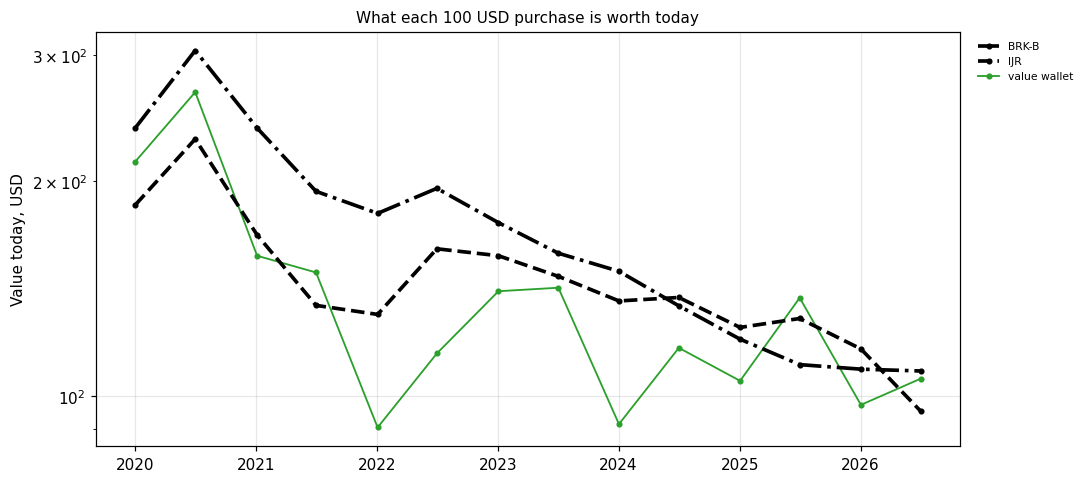
\includegraphics[width=1\textwidth]{yearly.png}
\caption{What each purchase is worth today, by date of purchase, on a logarithmic scale.}
\label{fig:yearly}
\end{figure}
\section{Value over time}
\begin{table}[H]
\centering
\small
\caption{Money put in and value today per start year (USD), and the money-weighted return a year.}\label{tab:value}
\begin{tabular}{l l r r r r}
\hline
Start & Holder & Put in & Value & Multiple & A year \\
\hline
2016 & Value wallet & 1,400 & 1,928 & 1.38 & 8.9\% \\
 & Value wallet with sells & 1,400 & 1,887 & 1.35 & 8.3\% \\
 & S\&P SmallCap 600 & 1,400 & 2,052 & 1.47 & 10.6\% \\
 & Berkshire Hathaway & 1,400 & 2,415 & 1.73 & 15.2\% \\
\hline
2020 & Value wallet & 1,400 & 1,928 & 1.38 & 8.9\% \\
 & Value wallet with sells & 1,400 & 1,887 & 1.35 & 8.3\% \\
 & S\&P SmallCap 600 & 1,400 & 2,052 & 1.47 & 10.6\% \\
 & Berkshire Hathaway & 1,400 & 2,415 & 1.73 & 15.2\% \\
\hline
2023 & Value wallet & 800 & 936 & 1.17 & 7.7\% \\
 & Value wallet with sells & 800 & 936 & 1.17 & 7.7\% \\
 & S\&P SmallCap 600 & 800 & 1,044 & 1.30 & 13.1\% \\
 & Berkshire Hathaway & 800 & 1,066 & 1.33 & 14.2\% \\
\hline
2025 & Value wallet & 400 & 446 & 1.11 & 10.4\% \\
 & Value wallet with sells & 400 & 446 & 1.11 & 10.4\% \\
 & S\&P SmallCap 600 & 400 & 465 & 1.16 & 14.8\% \\
 & Berkshire Hathaway & 400 & 449 & 1.12 & 11.1\% \\
\hline
\end{tabular}
\end{table}
Table \ref{tab:value} and Figure \ref{fig:value} follow the four investors. Each puts in 100 USD every January and July from the start year; the value wallet never sells. The return a year is money-weighted: the constant yearly rate that turns the payments into today's value.

The investor who started in 2016 earns 8.9\% a year against 10.6\% in the S\&P SmallCap 600 and 15.2\% in Berkshire Hathaway. From 2020 the rates are 8.9\%, 10.6\% and 15.2\%; from 2023 7.7\%, 13.1\% and 14.2\%; from 2025, over less than two years, 10.4\%, 14.8\% and 11.1\%. The wallet's value swings more than either comparison, because five companies of a few industries are far less diversified than the index or Berkshire.

The value wallet with sells buys the same picks with the same money, but at each decision it also sells part of any holding whose score has fallen; Section \ref{sec:selling} describes the rule. From 2016 it is worth 1,887 USD (8.3\% a year), from 2020 1,887 USD (8.3\%) and from 2025 446 USD (10.4\%).

\begin{figure}[H]
\centering
\begin{subfigure}[t]{0.480\textwidth}
\centering
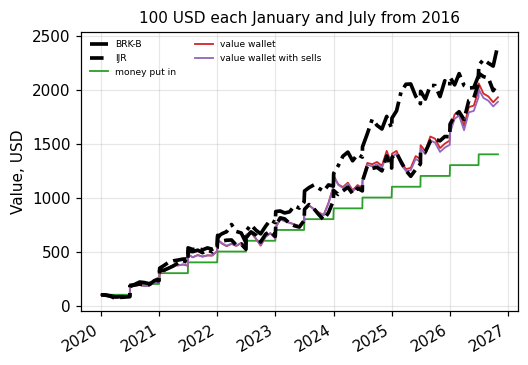
\includegraphics[width=\linewidth]{value_2016.png}
\caption{From 2016}
\end{subfigure}\hfill
\begin{subfigure}[t]{0.480\textwidth}
\centering
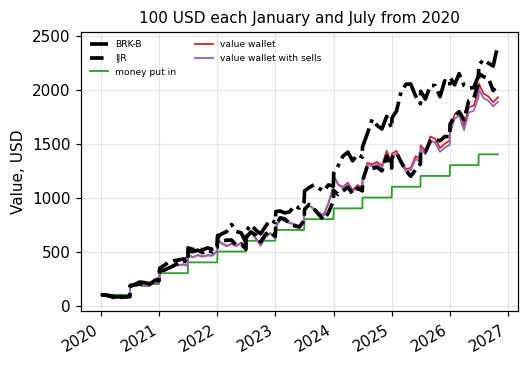
\includegraphics[width=\linewidth]{value_2020.png}
\caption{From 2020}
\end{subfigure}\hfill
\par\medskip
\begin{subfigure}[t]{0.480\textwidth}
\centering
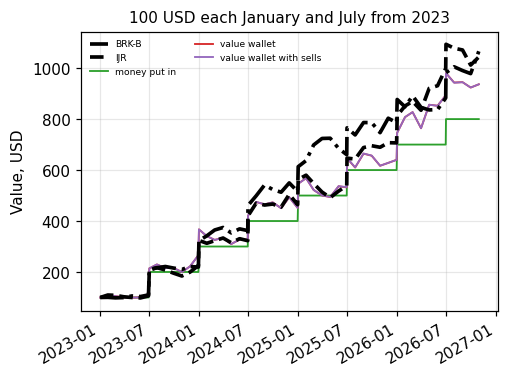
\includegraphics[width=\linewidth]{value_2023.png}
\caption{From 2023}
\end{subfigure}\hfill
\begin{subfigure}[t]{0.480\textwidth}
\centering
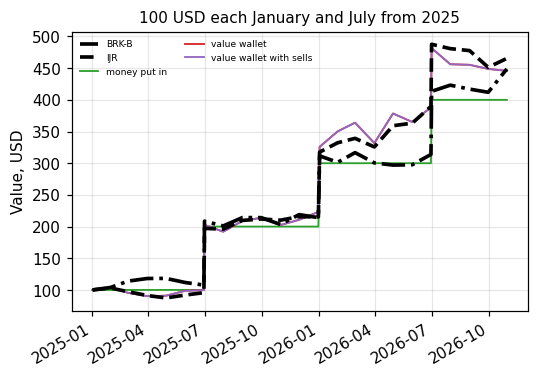
\includegraphics[width=\linewidth]{value_2025.png}
\caption{From 2025}
\end{subfigure}\hfill
\caption{Value of 100 USD every January and July from each start year, in USD, next to the money put in; the S\&P SmallCap 600 dashed and Berkshire Hathaway dash-dot.}
\label{fig:value}
\end{figure}
\section{Selling below the threshold}
\label{sec:selling}
\begin{table}[H]
\centering
\small
\caption{Sales of the investor who started in 2020: share of each holding sold, its score on the 0-to-1 scale, and the proceeds.}\label{tab:sales}
\begin{tabular}{l p{11cm} r}
\hline
Year & Sold: share of the holding (score) & Proceeds, USD \\
\hline
2021-01 & SCSC 9\% (score 0.37) & 3.13 \\
2021-07 & GVA 13\% (score 0.35), SCSC 12\% (score 0.35) & 14.18 \\
2022-01 & GVA 13\% (score 0.35) & 8.38 \\
2024-01 & GIII 8\% (score 0.37) & 6.51 \\
2025-01 & GVA 5\% (score 0.38) & 6.36 \\
2026-01 & MTRN 2\% (score 0.39) & 0.74 \\
2026-07 & GVA 4\% (score 0.39), MTRN 1\% (score 0.40) & 8.92 \\
\hline
\end{tabular}
\end{table}
Each January and July, before buying, the wallet with sells checks every company it holds. The score is put on a scale from 0 to 1, the share of the most the company could score on the rules it is measured on. A holding scoring 0.4 or less is sold in part: the share sold is (0.4 less the score) divided by 0.4, so all of it at a score of 0 and almost none just under 0.4. Holdings are sold, never sold short. The proceeds are added to the decision's 100 USD and buy its picks. Table \ref{tab:sales} lists the 9 sales of the investor who started in 2020, worth 48 USD in all.

\section{Wallet contents}
Figure \ref{fig:contents} follows every company in the wallet with sells of the investor who started in 2020, month by month. A line starts or steps up when the company is bought, steps down when part of it is sold, and rises or falls with the price in between. The dashed lines follow the same money in the S\&P SmallCap 600 and in Berkshire Hathaway, divided by the number of companies the wallet holds on the date, so they show what one holding would be worth in the index or in Berkshire. Appendix \ref{app:contents} gives each holding's value after every January's trades, the money put in and the proceeds of sales.

\begin{figure}[H]
\centering
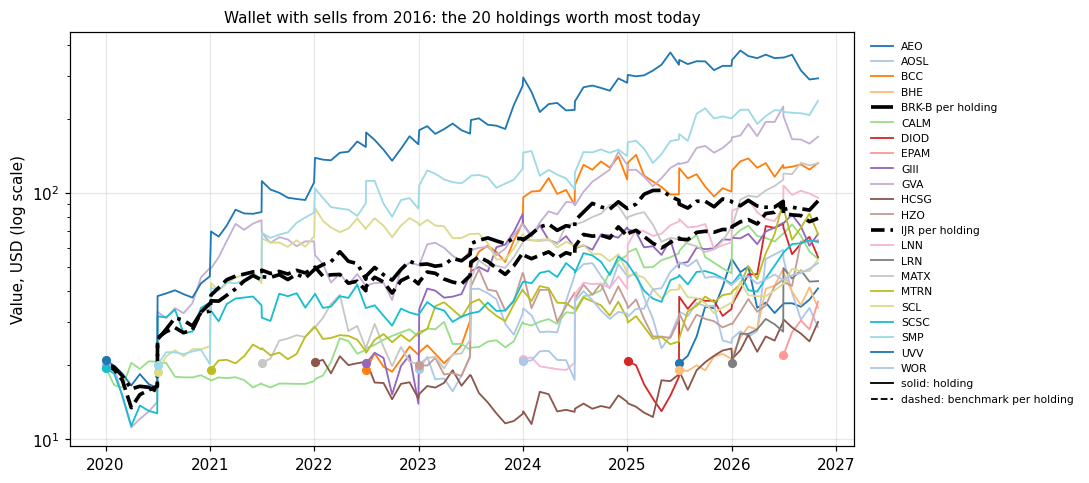
\includegraphics[width=1\textwidth]{contents.png}
\caption{Value of each holding in the wallet with sells (solid) and of the S\&P SmallCap 600 and Berkshire Hathaway divided by the number of holdings (dashed), in USD on a logarithmic scale.}
\label{fig:contents}
\end{figure}
\section{Rules behind the winners}
\begin{table}[H]
\centering
\small
\caption{Dollars ahead of the same money in the S\&P SmallCap 600, per pick: total, average and median of the picks that beat the index and of those that lagged it.}\label{tab:dollars}
\begin{tabular}{l r r r r}
\hline
Picks & Number & USD ahead, total & Average & Median \\
\hline
Beat the S\&P SmallCap 600 & 21 & +348 & +16.6 & +4.5 \\
Lagged the S\&P SmallCap 600 & 49 & -472 & -9.6 & -9.2 \\
\hline
All picks & 70 & -124 & -1.8 & -6.2 \\
\hline
\end{tabular}
\end{table}
Of the picks, 21 have done better than the S\&P SmallCap 600 since their purchase and 49 have not, but a count treats a large win and a small loss alike. Table \ref{tab:dollars} weighs them in dollars: each pick's value today less what the same money would be worth in the S\&P SmallCap 600. The winners are 348 USD ahead of the index and the laggards 472 USD behind, a net -124 USD, the wallet's whole lead over the index. The median winner is 4 USD ahead and the median laggard 9 USD behind; the average win is 1.7 times the average loss. The wins are concentrated: the 5 largest, GVA Jul 2020, GVA Jan 2020, MATX Jul 2021, MTRN Jan 2021 and MATX Jul 2023, make up 77\% of the winners' total.

Figure \ref{fig:rules} compares the mean points per rule of the winners and of the laggards on the day they were picked, each pick weighted by its dollars ahead or behind the index, so the large wins and losses count most; the rules are ordered by how much more the winners scored. The winners scored most above the others on 10-year earnings growth (G5), P/E times P/B (G7), price to tangible assets (E6) and 4-year earnings growth (E5); the picks that lagged scored higher on current ratio (lenient) (E1) and current ratio (G2a). With so few picks, these differences describe this sample; they do not establish which rules work. Appendix \ref{app:rules} explains each rule, and Appendix \ref{app:weighting} tests whether the rule weights favour the rules that told winners from losers.

\begin{figure}[H]
\centering
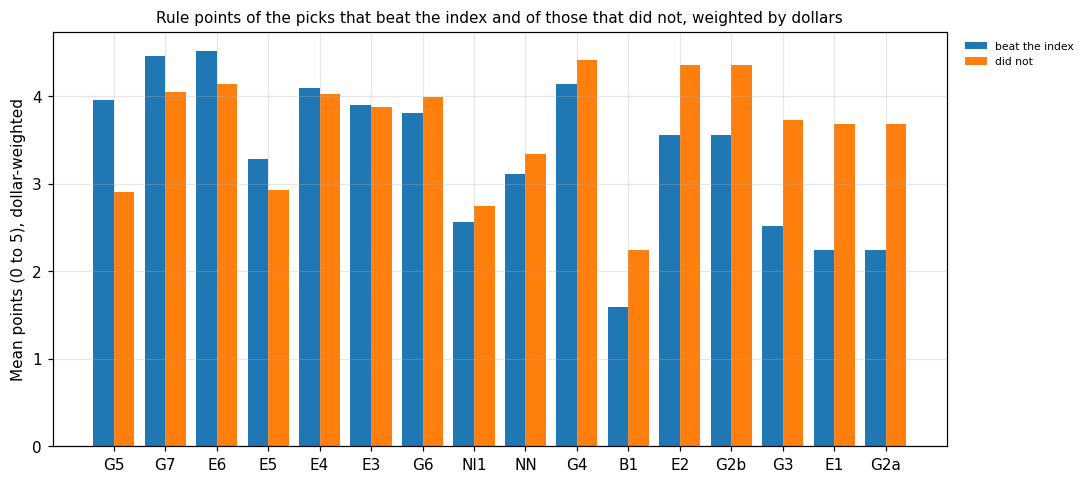
\includegraphics[width=1\textwidth]{rules.png}
\caption{Mean points per rule (0 to 5) of the picks that beat the S\&P SmallCap 600 since purchase and of those that did not, each pick weighted by its dollars ahead or behind the index.}
\label{fig:rules}
\end{figure}
\section{Price history of the picks}
Figure \ref{fig:pick-prices} shows the share price of every company the investor who started in 2023 bought or sold, and of the next picks, over the last 5 years. The price is split-adjusted and excludes dividends, as a price chart shows it; the companies run from the best to the worst price change over the 5 years, given beside each name; when they do not fit on one page, only the 5 best and the 5 worst are shown. Each purchase is marked in green and each sale in red, at the price on the decision date; a larger marker means more money. Figure \ref{fig:trade-amounts} gives the same trades in USD per company and decision date.

\begin{figure}[H]
\centering
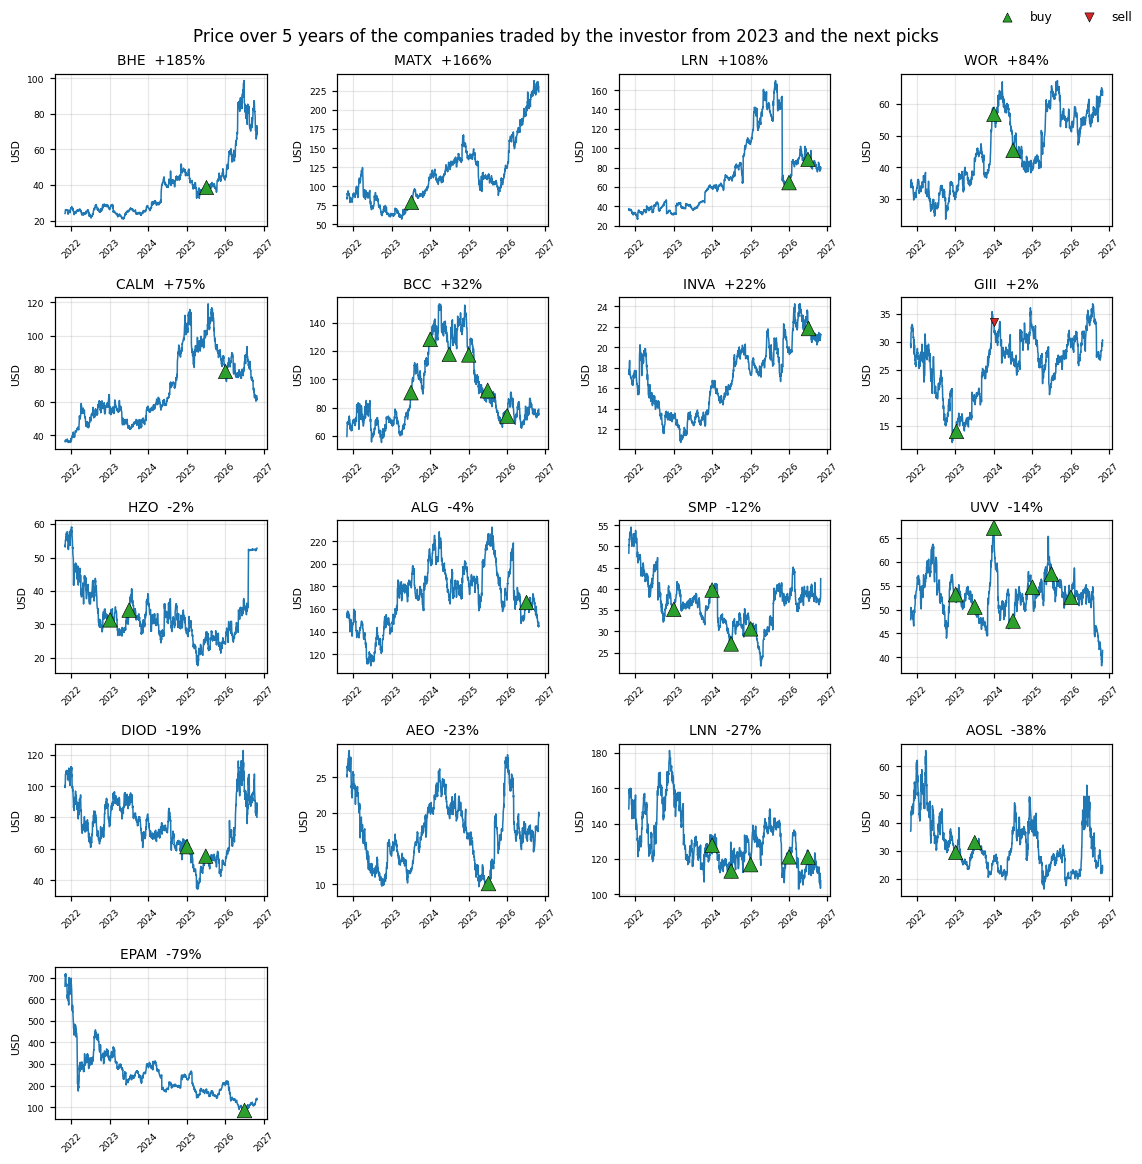
\includegraphics[width=1\textwidth]{pick_prices.png}
\caption{Share price (USD, split-adjusted, dividends excluded) over the last 5 years, one panel per company, ordered from the best to the worst price change over the period; purchases (green) and sales (red) of the investor who started in 2023, marker area in proportion to the USD traded.}
\label{fig:pick-prices}
\end{figure}
\begin{figure}[H]
\centering
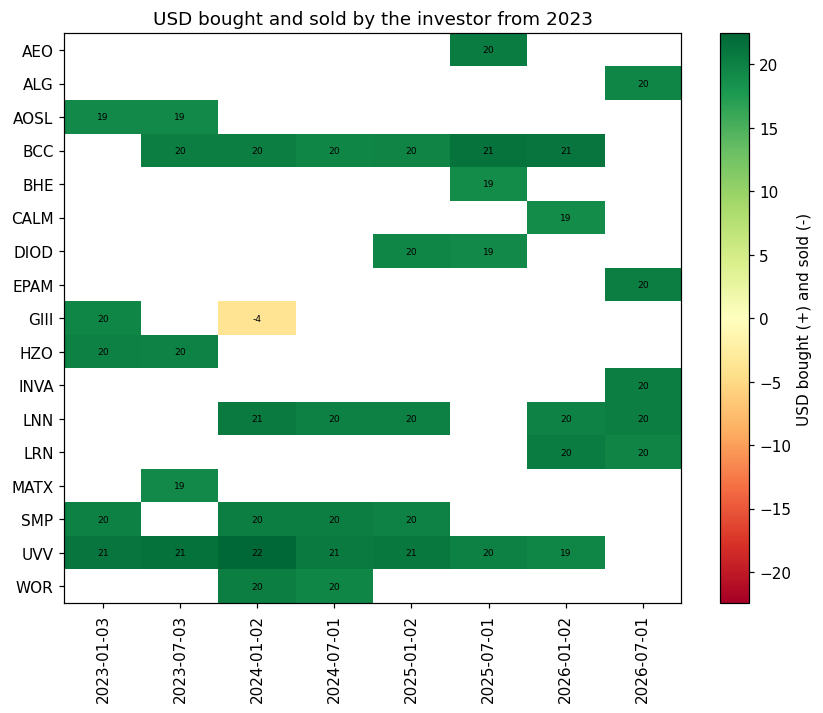
\includegraphics[width=1\textwidth]{trade_amounts.png}
\caption{USD bought (green, positive) and sold (red, negative) by the investor who started in 2023, per company and decision date.}
\label{fig:trade-amounts}
\end{figure}
\section{The next picks}
\begin{table}[H]
\centering
\small
\caption{The next picks on the latest score date: score, score on the 0-to-1 scale, weight and USD of each 100 USD.}\label{tab:next}
\begin{tabular}{l l r r r r}
\hline
Company & Sector & Score & Score 0 to 1 & Weight & USD \\
\hline
Lindsay Corporation (LNN) & Materials & 41.8 & 0.80 & 20.7\% & 20.65 \\
Innoviva, Inc. (INVA) & Health care & 41.5 & 0.84 & 20.5\% & 20.47 \\
Boise Cascade (BCC) & Industrials & 39.9 & 0.82 & 19.7\% & 19.70 \\
Alamo Group (ALG) & Industrials & 39.7 & 0.76 & 19.6\% & 19.60 \\
Stride, Inc. (LRN) & Discretionary & 39.6 & 0.81 & 19.6\% & 19.58 \\
\hline
\end{tabular}
\end{table}
On the latest score date, 18 September 2026, the five highest-scoring companies are Lindsay Corporation (LNN), Innoviva, Inc. (INVA), Boise Cascade (BCC), Alamo Group (ALG) and Stride, Inc. (LRN) (Table \ref{tab:next}). Each would receive its share of the next decision's 100 USD and of any proceeds from sales. The decision is taken on the first trading day of January with the scores known then, which include the annual reports filed until that day; these picks are a preview and may change. Figure \ref{fig:next-prices} shows each pick's share price over the last 5 years, with the earlier purchases of the investor who started in 2023 and the potential purchase at today's price.

\begin{figure}[H]
\centering
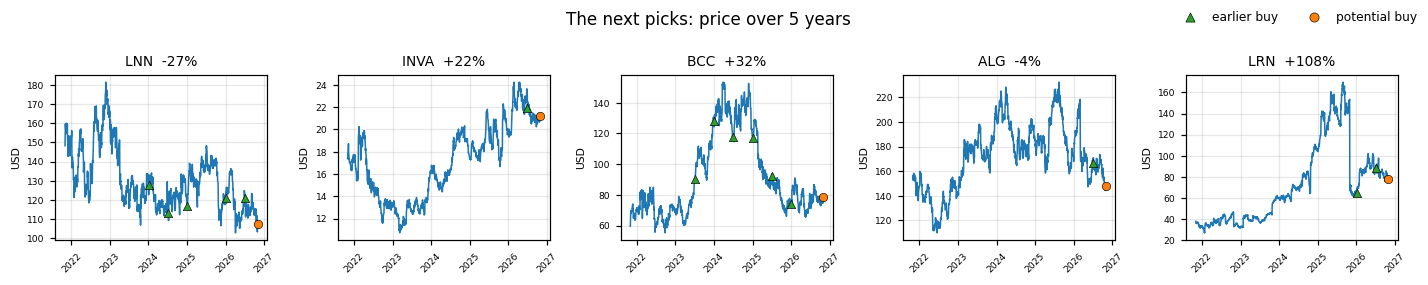
\includegraphics[width=1\textwidth]{next_prices.png}
\caption{Share price of each next pick (USD, split-adjusted, dividends excluded) over the last 5 years: earlier purchases of the investor who started in 2023 in green, the potential purchase at the latest price in orange.}
\label{fig:next-prices}
\end{figure}
\subsection{Sell check}
\begin{table}[H]
\centering
\small
\caption{Holdings the rule would sell in part: value today, score on the 0-to-1 scale, share to sell and amount.}\label{tab:sell}
\begin{tabular}{l r r r r}
\hline
Company & Holding, USD & Score 0 to 1 & Sell & Sell, USD \\
\hline
MarineMax, Inc. (HZO) & 64.21 & 0.37 & 7\% & 4.28 \\
\hline
\end{tabular}
\end{table}
The investor who started in 2020 holds 26 companies. With the scores of 18 September 2026, the rule would sell part of MarineMax, Inc. (HZO), 7\%, and keep the other 25 as they are (Table \ref{tab:sell}).

\section{Conclusions}
In this sample, the value picks bought twice a year and held are worth more today than the same money in the S\&P SmallCap 600 or in Berkshire Hathaway for each of the four start years. That describes the past under rules and settings chosen while looking at it; it is not a test of the strategy. The lead is uneven: the 13 purchases of Universal Corporation (UVV) make up 15\% of the 2020 investor's value, and the purchases of January 2021, January 2022, July 2022, January 2023, July 2023, January 2024, July 2024, January 2025 and January 2026 trail the index.

Before the strategy is used, three steps are needed: the companies that left the index must be added to the data, the score must be tested on more decisions (each quarter instead of each year), and trading costs and taxes must be included.

\newpage
\appendix
\section{Every purchase}
\label{app:purchases}
{\small
\begin{longtable}{l l l r r r r r r r}
\caption{Every purchase of the wallet with sells of the investor who started in 2020: weight in the decision's purchase, USD invested (the decision's 100 USD and the proceeds of sales), split-adjusted price at purchase and today, USD sold from it later, USD it keeps today and its total return with dividends, (sold + kept) / invested - 1.}\label{tab:purchases}\\
\hline
Year & Company & Sector & Weight & In & Bought at & Now & Sold & Kept & Return \\
\hline
\endhead
2020-01 & UVV & Staples & 21\% & 21 & 56.88 & 41.44 &  & 24 & +12\% \\
2020-01 & GVA & Industrials & 20\% & 20 & 27.59 & 123.62 & 13 & 68 & +306\% \\
2020-01 & LZB & Discretionary & 20\% & 20 & 31.04 & 30.44 &  & 23 & +13\% \\
2020-01 & CALM & Staples & 20\% & 20 & 42.02 & 63.56 &  & 38 & +96\% \\
2020-01 & SCSC & Technology & 19\% & 19 & 36.78 & 57.71 & 3 & 25 & +41\% \\
2020-07 & UVV & Staples & 22\% & 22 & 41.90 & 41.44 &  & 33 & +48\% \\
2020-07 & SMP & Discretionary & 20\% & 20 & 40.43 & 42.41 &  & 25 & +26\% \\
2020-07 & GVA & Industrials & 20\% & 20 & 17.94 & 123.62 & 19 & 101 & +514\% \\
2020-07 & SCSC & Technology & 19\% & 19 & 23.20 & 57.71 & 5 & 39 & +123\% \\
2020-07 & SCL & Materials & 19\% & 19 & 94.63 & 69.61 &  & 16 & -18\% \\
2021-01 & UVV & Staples & 23\% & 24 & 48.82 & 41.44 &  & 29 & +22\% \\
2021-01 & SMP & Discretionary & 21\% & 21 & 40.11 & 42.41 &  & 27 & +26\% \\
2021-01 & IOSP & Materials & 19\% & 20 & 89.56 & 99.89 &  & 24 & +21\% \\
2021-01 & MTRN & Materials & 19\% & 19 & 62.61 & 221.94 & 2 & 68 & +263\% \\
2021-01 & SCL & Materials & 18\% & 19 & 121.11 & 69.61 &  & 12 & -36\% \\
2021-07 & UVV & Staples & 24\% & 28 & 57.25 & 41.44 &  & 28 & +2\% \\
2021-07 & SMP & Discretionary & 20\% & 23 & 43.81 & 42.41 &  & 27 & +14\% \\
2021-07 & SCL & Materials & 19\% & 22 & 122.75 & 69.61 &  & 14 & -37\% \\
2021-07 & FELE & Industrials & 18\% & 21 & 81.08 & 95.38 &  & 26 & +24\% \\
2021-07 & MATX & Industrials & 18\% & 20 & 64.68 & 223.85 &  & 76 & +270\% \\
2022-01 & UVV & Staples & 24\% & 26 & 56.14 & 41.44 &  & 26 & +1\% \\
2022-01 & SMP & Discretionary & 20\% & 21 & 52.39 & 42.41 &  & 20 & -6\% \\
2022-01 & HCSG & Industrials & 19\% & 21 & 17.82 & 24.52 &  & 30 & +46\% \\
2022-01 & WGO & Discretionary & 19\% & 20 & 75.64 & 30.61 &  & 9 & -54\% \\
2022-01 & SCL & Materials & 19\% & 20 & 124.08 & 69.61 &  & 13 & -38\% \\
2022-07 & UVV & Staples & 22\% & 22 & 60.81 & 41.44 &  & 20 & -10\% \\
2022-07 & GIII & Discretionary & 20\% & 20 & 20.01 & 30.28 & 3 & 29 & +55\% \\
2022-07 & SMP & Discretionary & 20\% & 20 & 45.77 & 42.41 &  & 21 & +7\% \\
2022-07 & WGO & Discretionary & 19\% & 19 & 49.12 & 30.61 &  & 14 & -29\% \\
2022-07 & BCC & Industrials & 19\% & 19 & 60.58 & 78.83 &  & 30 & +55\% \\
2023-01 & UVV & Staples & 21\% & 21 & 53.18 & 41.44 &  & 21 & +0\% \\
2023-01 & SMP & Discretionary & 20\% & 20 & 35.17 & 42.41 &  & 27 & +37\% \\
2023-01 & HZO & Discretionary & 20\% & 20 & 31.38 & 52.76 &  & 34 & +68\% \\
2023-01 & GIII & Discretionary & 20\% & 20 & 13.97 & 30.28 & 4 & 40 & +121\% \\
2023-01 & AOSL & Technology & 19\% & 19 & 29.32 & 22.98 &  & 15 & -22\% \\
2023-07 & UVV & Staples & 21\% & 21 & 50.58 & 41.44 &  & 22 & +2\% \\
2023-07 & BCC & Industrials & 20\% & 20 & 90.57 & 78.83 &  & 20 & -3\% \\
2023-07 & HZO & Discretionary & 20\% & 20 & 34.30 & 52.76 &  & 31 & +54\% \\
2023-07 & AOSL & Technology & 19\% & 19 & 32.87 & 22.98 &  & 13 & -30\% \\
2023-07 & MATX & Industrials & 19\% & 19 & 79.13 & 223.85 &  & 56 & +193\% \\
2024-01 & UVV & Staples & 22\% & 23 & 67.18 & 41.44 &  & 17 & -25\% \\
2024-01 & LNN & Materials & 20\% & 21 & 127.69 & 107.63 &  & 18 & -13\% \\
2024-01 & BCC & Industrials & 20\% & 21 & 128.24 & 78.83 &  & 14 & -35\% \\
2024-01 & WOR & Industrials & 20\% & 21 & 56.72 & 62.75 &  & 24 & +15\% \\
2024-01 & SMP & Discretionary & 19\% & 21 & 39.74 & 42.41 &  & 24 & +17\% \\
2024-07 & UVV & Staples & 21\% & 21 & 47.64 & 41.44 &  & 21 & +2\% \\
2024-07 & SMP & Discretionary & 20\% & 20 & 27.04 & 42.41 &  & 34 & +70\% \\
2024-07 & LNN & Materials & 20\% & 20 & 113.16 & 107.63 &  & 20 & -2\% \\
2024-07 & WOR & Industrials & 20\% & 20 & 45.27 & 62.75 &  & 28 & +43\% \\
2024-07 & BCC & Industrials & 20\% & 20 & 117.69 & 78.83 &  & 14 & -29\% \\
2025-01 & UVV & Staples & 21\% & 22 & 54.70 & 41.44 &  & 19 & -14\% \\
2025-01 & LNN & Materials & 20\% & 21 & 116.77 & 107.63 &  & 20 & -6\% \\
2025-01 & SMP & Discretionary & 20\% & 21 & 30.59 & 42.41 &  & 31 & +47\% \\
2025-01 & BCC & Industrials & 20\% & 21 & 117.23 & 78.83 &  & 14 & -31\% \\
2025-01 & DIOD & Technology & 20\% & 21 & 61.31 & 80.13 &  & 27 & +31\% \\
2025-07 & BCC & Industrials & 21\% & 21 & 92.12 & 78.83 &  & 19 & -13\% \\
2025-07 & AEO & Discretionary & 20\% & 20 & 10.19 & 19.61 &  & 41 & +102\% \\
2025-07 & UVV & Staples & 20\% & 20 & 57.48 & 41.44 &  & 16 & -21\% \\
2025-07 & DIOD & Technology & 19\% & 19 & 55.30 & 80.13 &  & 28 & +45\% \\
2025-07 & BHE & Technology & 19\% & 19 & 38.77 & 68.37 &  & 34 & +79\% \\
2026-01 & BCC & Industrials & 21\% & 21 & 74.12 & 78.83 &  & 23 & +7\% \\
2026-01 & LRN & Discretionary & 20\% & 20 & 64.61 & 78.36 &  & 25 & +21\% \\
2026-01 & LNN & Materials & 20\% & 20 & 121.15 & 107.63 &  & 18 & -10\% \\
2026-01 & UVV & Staples & 19\% & 20 & 52.58 & 41.44 &  & 17 & -16\% \\
2026-01 & CALM & Staples & 19\% & 19 & 78.47 & 63.56 &  & 16 & -18\% \\
2026-07 & LNN & Materials & 20\% & 22 & 121.07 & 107.63 &  & 20 & -11\% \\
2026-07 & INVA & Health care & 20\% & 22 & 21.90 & 21.22 &  & 21 & -3\% \\
2026-07 & EPAM & Technology & 20\% & 22 & 85.24 & 140.51 &  & 36 & +65\% \\
2026-07 & LRN & Discretionary & 20\% & 22 & 88.57 & 78.36 &  & 19 & -12\% \\
2026-07 & ALG & Industrials & 20\% & 21 & 166.30 & 147.76 &  & 19 & -11\% \\
\hline
\end{longtable}}
\section{Wallet contents by year}
\label{app:contents}
\begin{table}[H]
\centering
\small
\caption{Wallet with sells of the investor who started in 2020: value of each holding after each January's trades and today (USD), and the money put in and the proceeds of sales to date, July decisions included.}\label{tab:contents}
\begin{tabular}{l r r r r r r r r }
\hline
Holding & 2020 & 2021 & 2022 & 2023 & 2024 & 2025 & 2026 & Now \\
\hline
LZB & 20 & 26 & 24 & 16 & 25 & 31 & 27 & 23 \\
UVV & 21 & 70 & 139 & 180 & 295 & 302 & 347 & 292 \\
CALM & 20 & 17 & 18 & 27 & 30 & 57 & 66 & 54 \\
SCSC & 19 & 33 & 39 & 32 & 44 & 52 & 43 & 63 \\
GVA & 20 & 49 & 56 & 51 & 74 & 124 & 168 & 169 \\
SMP &  & 41 & 104 & 107 & 146 & 161 & 202 & 237 \\
SCL &  & 43 & 87 & 74 & 67 & 46 & 36 & 54 \\
IOSP &  & 20 & 21 & 24 & 28 & 25 & 18 & 24 \\
MTRN &  & 19 & 29 & 27 & 40 & 30 & 40 & 68 \\
FELE &  &  & 24 & 21 & 25 & 26 & 26 & 26 \\
MATX &  &  & 28 & 20 & 65 & 80 & 73 & 132 \\
HCSG &  &  & 21 & 15 & 13 & 14 & 21 & 30 \\
WGO &  &  & 20 & 35 & 50 & 33 & 29 & 23 \\
BCC &  &  &  & 23 & 96 & 133 & 123 & 132 \\
GIII &  &  &  & 34 & 75 & 71 & 66 & 68 \\
AOSL &  &  &  & 19 & 34 & 45 & 26 & 29 \\
HZO &  &  &  & 20 & 47 & 34 & 29 & 64 \\
WOR &  &  &  &  & 21 & 31 & 43 & 52 \\
LNN &  &  &  &  & 21 & 62 & 85 & 96 \\
DIOD &  &  &  &  &  & 21 & 35 & 55 \\
BHE &  &  &  &  &  &  & 22 & 34 \\
AEO &  &  &  &  &  &  & 54 & 41 \\
LRN &  &  &  &  &  &  & 20 & 44 \\
INVA &  &  &  &  &  &  &  & 21 \\
EPAM &  &  &  &  &  &  &  & 36 \\
ALG &  &  &  &  &  &  &  & 19 \\
\hline
Put in & 100 & 300 & 500 & 700 & 900 & 1,100 & 1,300 & 1,400 \\
Sold & 0 & 3 & 26 & 26 & 32 & 39 & 39 & 48 \\
Total & 100 & 319 & 611 & 725 & 1,196 & 1,378 & 1,599 & 1,887 \\
\hline
\end{tabular}
\end{table}
\section{Testing the weighting}
\label{app:weighting}
\begin{table}[H]
\centering
\small
\caption{Each rule's weight w\_r on the picks' dates (overall, for the picks that beat the S\&P SmallCap 600 and for the others), the dollar-weighted mean points, the gap and the rank correlation with the return a year above the S\&P SmallCap 600.}\label{tab:weighting}
\begin{tabular}{l r r r r r r r}
\hline
Rule & w\_r & w\_r beat & w\_r not & Pts beat & Pts not & Gap & Corr. \\
\hline
NN & 1.00 & 1.00 & 1.00 & 3.11 & 3.34 & -0.23 & -0.06 \\
B1 & 0.97 & 0.97 & 0.97 & 1.59 & 2.24 & -0.64 & +0.04 \\
E6 & 0.96 & 0.95 & 0.96 & 4.51 & 4.14 & +0.37 & +0.25 \\
G6 & 0.80 & 0.79 & 0.81 & 3.81 & 3.99 & -0.18 & -0.03 \\
G7 & 0.70 & 0.69 & 0.71 & 4.46 & 4.05 & +0.41 & +0.11 \\
G4 & 0.68 & 0.68 & 0.68 & 4.14 & 4.41 & -0.27 & -0.42 \\
G2b & 0.61 & 0.61 & 0.60 & 3.56 & 4.36 & -0.80 & +0.09 \\
E2 & 0.57 & 0.57 & 0.57 & 3.56 & 4.36 & -0.80 & +0.09 \\
G3 & 0.57 & 0.57 & 0.57 & 2.52 & 3.73 & -1.22 & -0.20 \\
G5 & 0.52 & 0.51 & 0.52 & 3.96 & 2.90 & +1.05 & +0.05 \\
E4 & 0.51 & 0.51 & 0.51 & 4.10 & 4.03 & +0.07 & -0.18 \\
G2a & 0.47 & 0.48 & 0.47 & 2.24 & 3.69 & -1.45 & -0.34 \\
E3 & 0.46 & 0.46 & 0.46 & 3.90 & 3.87 & +0.02 & -0.01 \\
NI1 & 0.43 & 0.45 & 0.43 & 2.56 & 2.74 & -0.18 & +0.02 \\
E5 & 0.35 & 0.35 & 0.36 & 3.28 & 2.93 & +0.35 & -0.12 \\
E1 & 0.29 & 0.29 & 0.28 & 2.24 & 3.69 & -1.45 & -0.34 \\
\hline
\end{tabular}
\end{table}
Each rule's points are multiplied by its weight, one less the share of companies passing it on the date, so a rule few companies pass counts more. A good weighting gives most weight to the rules whose points went with better returns. Table \ref{tab:weighting} sets each rule's mean weight on the dates the picks were made against two measures of how well it told the 70 picks apart: the gap between the mean points of the picks that beat the S\&P SmallCap 600 and of those that did not, weighted by dollars as in Figure \ref{fig:rules}, and the rank correlation of the rule's points with each pick's return a year above the S\&P SmallCap 600. Figure \ref{fig:weighting} plots weight against gap; a good weighting puts its rules on a rising line, with the heavy rules above zero.

Across the rules, the rank correlation of weight and gap is +0.13, and of weight and correlation +0.40.

The weighting is unrelated to which rules worked. Weighted heavily but with a negative gap: debt to working capital (G2b), 20 years of dividends (G4), P/E (G6), debt to working capital (lenient) (E2), net-net (NN) and return on equity (B1). A positive gap but a light weight: 10-year earnings growth (G5), 5 years of profit (E3), current dividend (E4) and 4-year earnings growth (E5). Any change to the weights must be tested on years it was not fitted on.

\begin{figure}[H]
\centering
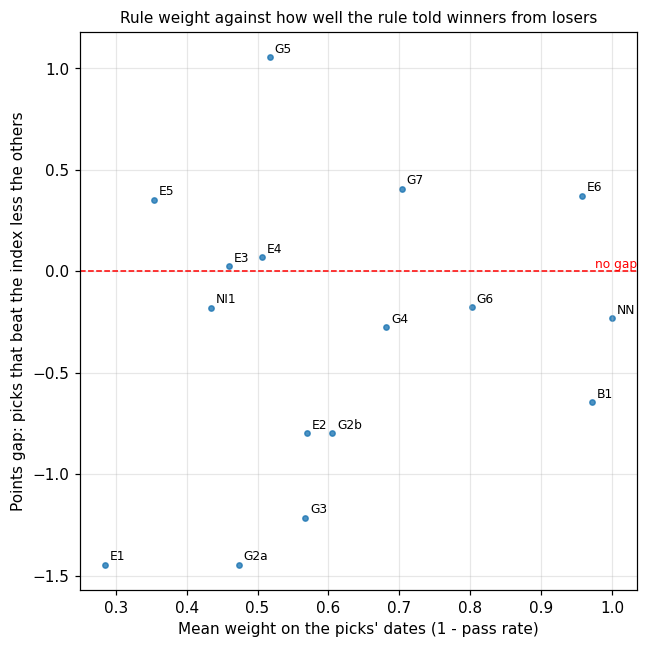
\includegraphics[width=0.6\textwidth]{weighting.png}
\caption{Each rule's mean weight against the gap in points between the picks that beat the S\&P SmallCap 600 and the others, weighted by dollars; rules above the line told winners from losers.}
\label{fig:weighting}
\end{figure}
\section{Forward information}
\label{app:lookahead}
\begin{table}[H]
\centering
\small
\caption{Truncation check: companies scored on the date, companies whose score differs when every input is cut at the date (per score), and whether the five picks are the same.}\label{tab:lookahead}
\begin{tabular}{l r r r r r l}
\hline
Date & Companies & Score & Score 0 to 1 & Unweighted & Share passed & Same picks \\
\hline
2018-12-21 & 0 & 0 & 0 & 0 & 0 & yes \\
2022-12-16 & 227 & 0 & 0 & 0 & 0 & yes \\
2025-12-19 & 367 & 0 & 0 & 0 & 0 & yes \\
\hline
\end{tabular}
\end{table}
A score must use only what was known on its date. Four guards are built in. A company's figures count from the day its annual report was filed with the SEC, and of all the figures filed for a year only the first reported is used, never a later restatement. Prices are the close on the scoring date and dividends are counted by their ex-date. Each January and July purchase uses the scores of the rebalance date two weeks before it. Rule weights come from the companies on the date alone.

These guards are tested by cutting every input at a date as if it were that day (filings filed on or before it, prices and dividends up to it), scoring the companies again and comparing the scores with the full run (Table \ref{tab:lookahead}). Any difference means information from after the date reached a score. On 21 December 2018, 16 December 2022 and 19 December 2025 the picks were the same, and the scores were identical on 21 December 2018, 16 December 2022 and 19 December 2025. The same check runs as a unit test. A rule whose window reaches back further than a company's price history (the 20-year dividend record of a younger company) is not evaluated rather than failed.

Three sources of forward information are outside this test. Only today's S\&P SmallCap 600 members are scored. The index's list gives no entry dates: a company counts from its latest addition in the list of changes, or from the start of that list (December 2019) when no addition is listed. The list holds selected changes only, so some companies count before they joined: a look-ahead that flatters the results. Companies that later left the index are missing, which flatters every result. Sectors are today's, used to leave out Financials and Real Estate in earlier years. And the score's design and settings were chosen while looking at 2016 to 2026, so no period tests it fairly: 2022 onwards, once meant as a held-out test, was used to choose between models.

\subsection{Companies missing from the data}
\begin{table}[H]
\centering
\small
\caption{Companies that left the S\&P SmallCap 600 since each start year, all missing from the data: in all, on their market value, and through an acquisition or another reason.}\label{tab:survivors}
\begin{tabular}{l r r r}
\hline
Start & Left the index & On market value & Acquired or other \\
\hline
2016 & 491 & 21 & 470 \\
2020 & 487 & 21 & 466 \\
2023 & 318 & 17 & 301 \\
2025 & 147 & 0 & 147 \\
\hline
\end{tabular}
\end{table}
Table \ref{tab:survivors} counts the companies that left the S\&P SmallCap 600 after each start year; none of them is in the data, of any sector. Most left through an acquisition, often at a premium; those that dropped out on their market value are the likely losers a real investor could have picked. The later the start, the fewer are missing, which is why the investor who started in 2020 is the reference of this report. The count starts with the index's list of changes, which begins in December 2019: removals before that are not counted, so for earlier start years it understates the gap. The bias is removed only when the historical members of the index are added to the data.

\section{The rules}
\label{app:rules}
\begin{table}[H]
\centering
\small
\caption{The rules: what each measures, the better direction and when a company passes.}\label{tab:rules}
\begin{tabular}{l p{2.2cm} p{5.2cm} l p{2.8cm}}
\hline
Rule & Name & What it measures & Better & Passes when \\
\hline
G2a & current ratio & Current assets divided by current liabilities: what the company owns against what it owes within a year. & higher & at least 2.0 \\
G2b & debt to working capital & Long-term debt divided by net current assets (current assets less current liabilities). & lower & at most 1.0 \\
G3 & 10 years of profit & Number of the last 10 fiscal years with positive earnings per share. & higher & all 10 years \\
G4 & 20 years of dividends & Number of the 20 calendar years before the decision in which a dividend was paid. & higher & all 20 years \\
G5 & 10-year earnings growth & Average earnings per share of the last 3 years over the average of 3 years a decade earlier. & higher & at least 1.33 \\
G6 & P/E & Price over the average earnings per share of the last 3 years. & lower & at most 15.0 \\
G7 & P/E times P/B & P/E as in G6 times the price over book value per share. & lower & P/B at most 1.5, or the product at most 22.5 \\
E1 & current ratio (lenient) & Current ratio, as G2a. & higher & at least 1.5 \\
E2 & debt to working capital (lenient) & Long-term debt over net current assets, as G2b. & lower & at most 1.1 \\
E3 & 5 years of profit & Number of the last 5 fiscal years with positive earnings per share. & higher & all 5 years \\
E4 & current dividend & Dividends paid over the last 365 days, as a yield on the price. & higher & any dividend \\
E5 & 4-year earnings growth & Change in earnings per share over 4 years, relative to the earlier figure. & higher & earnings per share grew \\
E6 & price to tangible assets & Market value over net tangible assets (equity less goodwill and other intangible assets). & lower & at most 1.2 \\
NN & net-net & Market value over net current asset value (current assets less all liabilities). & lower & at most 0.67 \\
B1 & return on equity & Number of the last 10 years with return on equity (net income over equity) of at least 15\%. & higher & at least 7 years, and long-term debt at most 0.5 times equity \\
NI1 & net income growth & Growth of net income from the year before to the latest year. & higher & net income grew \\
\hline
\end{tabular}
\end{table}
Table \ref{tab:rules} explains each rule: what it measures, whether a higher or a lower value earns more points, and when a company passes it. The points come from the company's rank on the measure among all companies on the date; the pass threshold sets the rule's weight. Rules G follow Graham's defensive investor (The Intelligent Investor, chapter 14), rules E his enterprising investor (chapter 15) and his net-net test (NN), B1 Buffett's return on equity, and NI1 was added for net income growth. Two pairs test the same measure at different strictness (G2a and E1, G2b and E2), so the current ratio and debt count twice.

\end{document}
